\documentclass[12pt]{article}
\usepackage[latvian]{babel}
\usepackage[left=3cm,top=2cm,right=2cm,bottom=2cm]{geometry}
\usepackage{graphicx}
\usepackage{float}
\usepackage{titletoc}
\usepackage{caption}
\usepackage{biblatex}
\usepackage{sectsty}
\sectionfont{\centering}
\title{Music Overflow}

\addto\captionslatvian{\renewcommand{\figurename}{Diagramma}}

\begin{document}

\begin{titlepage}
	\begin{center}
		\vspace*{1cm}
 
       Latvijas Universitāte \\
       Datorzinātņu Fakultāte
 
       \vspace{1.5cm}
 
       \textbf{\huge{Music Overflow}}
       
       \vspace{3cm}
       Noslēguma darbs \\
       Programminženierijā
 

	\end{center}
\end{titlepage}

\textbf{\large Anotācija}

Darba autori:
\begin{itemize}
	\setlength{\itemsep}{0em}
	\item Deina Banka
	\item Edgars Lauks
	\item Jeļizaveta Zaharova
	\item Margarita Parhomenko
	\item Toms Bēmis
\end{itemize}

\indent Darba nosaukums: ``Music Overflow''.\\
\indent Darba veids: programmatūras prasības specifikācija (PPS).\\
\indent Studiju programma: Datorzinātnes.\\
\indent Darba zinātniskais vadītājs: Maksims Kravcevs.\\

Šī darba mērķis ir izveidot programmas prasības specifikāciju (PPS), kas apraksta sistēmu ``Music Overflow''.
Sistēma ``Music Overflow'' ir lietotne, kura palīdz lietotājiem iegūt orģinālo dziesmas nosaukumu, ja ir zināma tikai melodija, uzklausot citu lietotāju minējumus. ``Music Overflow'' sniedz iespēju veidot jautājumus, kuros iespējams atdarināt melodiju, kas dotu pietiekošu informāciju par orģinālo dziesmu, kā arī apmainīties ar sevis radītām melodijām un komentāriem par tām. Sistēma arī glabā lietotāju ievadītās melodijas, datus un saites uz attiecīgo skaņdarbu, ja atrasts. \\
\indent Darbs sastāv no 3 daļām. Tā pirmajā daļā ir sistēmas lietotāju apraksts un tās projektējums, sistēmas ierobežojumi, pieņēmumi un atkarības. Otrajā daļā ir datu bāzes apraksts un funkcionālās un nefunkcionālās prasības sistēmai. Trešajā daļā doti datu bāzes, funkciju, un lietotāja saskarņu projektējumi. \\
\indent Rezultātā izstrādāta programmas prasības specifikācija, ar kuru palīdzību var izveidot funkcionējošo sistēmu ``Music Overflow''. \\
\indent Darbs kopumā izklāstīts ... lappusēs, tajā iekļautas ... tabulas un ... diagrammas.  Darbā izmantoti ... literatūras avoti un pievienoti ... pielikumi.

Atslēgas vārdi: mūzika, melodija

\pagebreak

\textbf{\large Abstract}\\
\indent Authors:
\begin{itemize}
	\setlength{\itemsep}{0em}
	\item Deina Banka
	\item Edgars Lauks
	\item Jeļizaveta Zaharova
	\item Margarita Parhomenko
	\item Toms Bēmis
\end{itemize}

Project name: ``Music Overflow''\\
Project type: Software Requirements Specification (SRS)\\
Program: Computer Science\\
Supervisor: Maksims Kravcevs\\

Goal of this project is to create a software requirements specification, which describes the system ``Music Overflow''. System ``Music Overflow'' is an application, which helps users to find the title of an original song, by knowing only the melody, by reading the guesses of other users. ``Music Overflow'' offers to create questions, in which it is possible to recreate a melody, which would give enough information about the original song, and to create original melodies to share and give comments about. System also stores user created melodies, data and links to the correct composition, if found.\\
\indent The project consists of 3 parts. The first part consists of description of the system's users and it's design, limitations of the system, assumptions and dependencies. Second part consists of description of the database and functional and non-functional requirements for the system. Third part consists of database, function and user interface designs.\\
\indent As a result a systems requirement specification has been designed, with which a functional system ``Music Overflow'' can be developed.\\
\indent The project consists of ... pages, it has .. tables and ... diagrams. ... sources have been used and ... attachments added.\\
\indent Keywords: music, melody

\pagebreak

\tableofcontents

\pagebreak

\section*{Ievads}
\addcontentsline{toc}{section}{Ievads}

\textbf{Nolūks}

Šī programmatūras prasību specifikācija (PPS) ir izstrādāta un paredzēta lietotnes „Music Overflow” prasību aprakstīšanai.
Šī programmatūras prasību specifikācijas izstrādāšanas nolūks ir precīzi aprakstīt būtiskākās programmatūras darbības funkcijas, to prasības un iespējas, kā arī lietotāja saskarņu prasības, lai pēc specifikācijas izstrādes ir iespējama tālāka lietotnes galīgā izstrāde lietotājam izmantojamā veidā.
Lietotnes nolūks ir palīdzēt atrast dziesmas nosaukumu, no kuras atceras tikai melodijas daļu.
Atbilstoši šai specifikācijai tiks izstrādāta sistēma. Šis dokuments ir savstarpēja vienošanās starp pasūtītāju un izpildītāju. Šajā prasību specifikācijā tiek noformulētas sistēmas prasības un raksturota funkcionalitāte.



\textbf{Darbības sfēra}

Sistēma ``Music Overflow'' ir lietotne, kura glabā lietotāju ievadītās melodijas, datus un saites uz attiecīgo skaņdarbu. Šī lietotne sniedz lietotājiem iespēju veidot jautājumus, kuros iespējams atdarināt mūzikas ierakstu, ievadot ritmu, kas dod pietiekošu informāciju par orģinālo dziesmu, kā arī apmainīties ar sevis radītām melodijām un komentāriem par tām.


\textbf{Saistība ar citiem dokumentiem}

Dokumenta noformēšanā ievērotas standarta LVS 68:1996 ``Programmatūras prasību specifikācijas ceļvedis'' prasības.

\textbf{Pārskats}\\
Dokuments sastāv no 5 daļām:
\begin{itemize}
\item Pirmajā daļā (1.nodaļā) ir ievadinformācija, kas satur dokumenta nolūku, mērķi, definīciju skaidrojumu, citu dokumentu izmantošana dokumenta tapšanas laikā;
\item Otrajā daļā tiek dots ieskats, par vispārējo produkta struktūru, kā funkcijas, ierobežojumi , kā arī atkarības, no citiem faktoriem;
\item Trešajā daļā tiek norādītas funkcionālās prasības uz izstrādājamo programmu;
\item Ceturtajā daļā aprakstītas saskarnes prasības;
\item Piektajā daļā aprakstītas nefunkcionālās prasības uz izstrādājamo produktu.
\end{itemize}

\section*{Apzīmējumu saraksts}
\addcontentsline{toc}{section}{Apzīmējumu saraksts}

\noindent Atbilde - Lietotāja ievadīts teksts, kas referencē uzdotu jautājumu.\\
Komentārs - Lietotāja ievadīts teksts, kas referencē kādu atbildi par uzdoto jautājumu.\\
Vērtējums - Lietotāju atzinums par to, cik pareiza vai nepareiza ir kāda atbilde.\\
URL - (angļu val.)``Unified Resource Locator'' - ``Vienotais Resursu Vietrādis'' jeb tīmekļa adrese.\\
Oauth - atvērtais standarts autorizācijas resursu deleģēšanai.\\

\pagebreak

\section{Vispārējais apraksts}

\subsection{Esošā stāvokļa apraksts}

Jaunas tīmekļa lietojumprogrammas izstrāde, mūzikas ierakstu atdarināšanai un orģinālo autoru un autordarbu identificēšanai.

\subsection{Pasūtītājs}

Sistēma aprakstīta pēc studentu grupas iniciatīvas programminženierijas kursa ietvaros.

\subsection{Produkta perspektīva}

Uzturēt saiti starp sistēmas lietotājiem un informāciju mūzikas datubāzēs. Ērti izveidot melodijas, piemeklēt tām esošus skaņdarbus, dalīties ar mūzikas ierakstiem un viedokļiem par tiem vienotā integrālā sistēmā.

\subsection{Darījumprasības}
\begin{itemize}
\item Sniegt lietotājiem iespēju veidot jautājumus, kuros iespējams atdarināt mūzikas ierakstu, kas dod pietiekošu informāciju par orģinālo dziesmu
\item Piedāvāt lietotājiem atrisināt citu lietotāju uzdotos jautājumus, lai veiksmīgi atrastu ieraksta autoru vai dziesmas nosaukumu
\item Informēt lietotājus, ļaut tiem sazināties savā starpā un paziņot par veiksmīgi atrastu izpildītāju un dziesmu
\item Dot iespēju mūzikas izpildītājiem tikt atpazītiem starp patērētājiem, neaizskarot autortiesības.
\item Sniegt lietotājiem iespēju dalīties ar mūziku caur Facebook.
\end{itemize}

\subsection{Sistēmas lietotāji}

Lietojumprogramma pieejama tikai izmantojot pārlūkprogrammu. Lietotājam ir nepieciešamas pamatzināšanas mūzikā, kā arī ir nepieciešama prasme darbam ar datoru un ar uzstādīto interneta pārlūkprogrammu. Administratoram nav nepieciešamas specifiskas mūzikas zināšanas, bet ir nepieciešamas datu apstrādes zināšanas.\\

\begin{center}
\begin{tabular}{|c|c|}
\hline
Administrators & Jauna lietotāja pievienošana  \\
& Lietotāja visas informācijas izdzēšana \\
& Komentāru rediģēšana \\
\hline
Reģistrēts lietotājs & Ritma ievadīšana \\
& Nošu pievienošana \\
& Konta dzēšana \\
& Dalīšanās ar savu melodiju\\
\hline
Nereģistrēts lietotājs & Konta izveidošana \\
& Ritma ievadīšana \\
& Nošu pievienošana \\
\hline
\end{tabular}
\captionof{table}{Lietotāju lomas}
\end{center}

\begin{figure}[H]
\begin{center}
		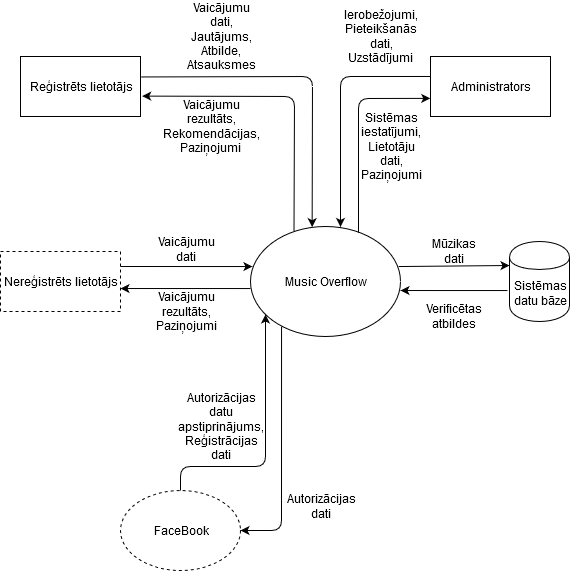
\includegraphics[scale=0.5]{DPD0.png}
		\caption{Datu plūsmas 0. līmeņa diagramma}
		\label{fig:dpd_0}
\end{center}
\end{figure}

\subsection{Vispārējie ierobežojumi}

\begin{itemize}
\item Sistēmas darbināšanai jābūt bez instalēšanas un izmantojot pārlūkprogrammu.
\item Sistēmas darbībai jābūt atbalstītai uz trim populārākajām pārlūkprogrammām: FireFox, Chrome, Safari.
\item Prasību apkopošanas laikā netika identificēti faktori, kuru izmaiņas var atstāt iespaidu uz prasību realizāciju.
\item Nepieciešams aizsargāt autortiesības par oriģinālo melodiju.
\item Laika ierobežojums melodijas ievadīšanai.
\end{itemize}

\subsection{Pieņēmumi un atkarības}

Pieeja publicēt jautājumus nepieciešama autentifikācija izmantojot trešo personu autentifikācijas informāciju, vai izveidoto kontu lietojumprogrammā. Lietotājam nepieciešams veids kā atskaņot audio. Pārlūkprogrammai nepieciešams HTML tehnoloģijas atbalsts, priekš lietotāja ievades rīka mūzikas atdarināšanai.

\section{Programmatūras prasību specifikācija}

\subsection{Konceptuālais datu bāzes apraksts}

\begin{figure}[H]
	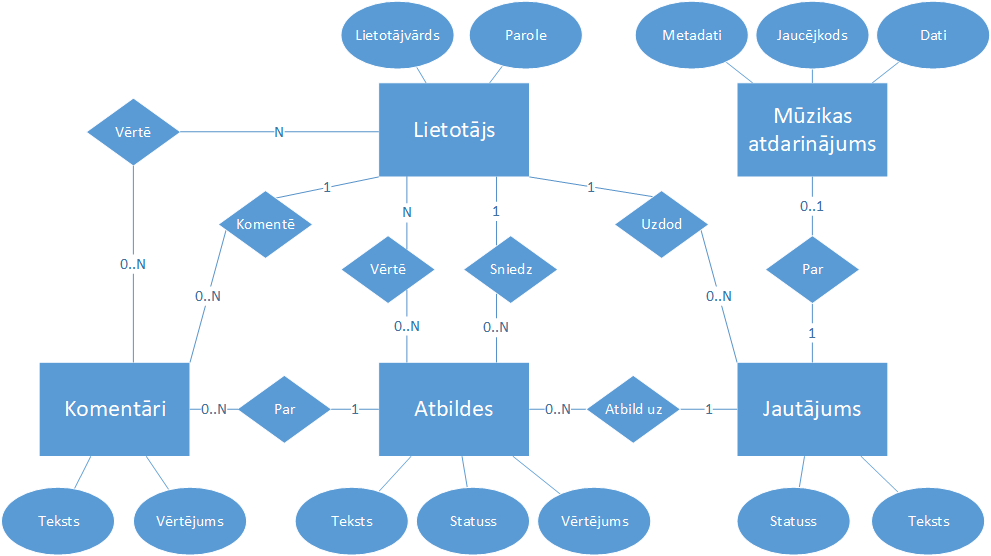
\includegraphics[width=\linewidth]{DB_concept.png}
	\caption{Datubāzes konceptuālais modelis}
	\label{fig:db_konceptualais}
\end{figure}

\subsection{Funkcionālās prasības}

\subsubsection{Vispārējās nodaļas, kas saistītas ar funckiju aprakstīšanu}

\subsubsection{Funkciju sadalījums pa moduļiem/komponentiem}

\begin{figure}[H]
\begin{center}
	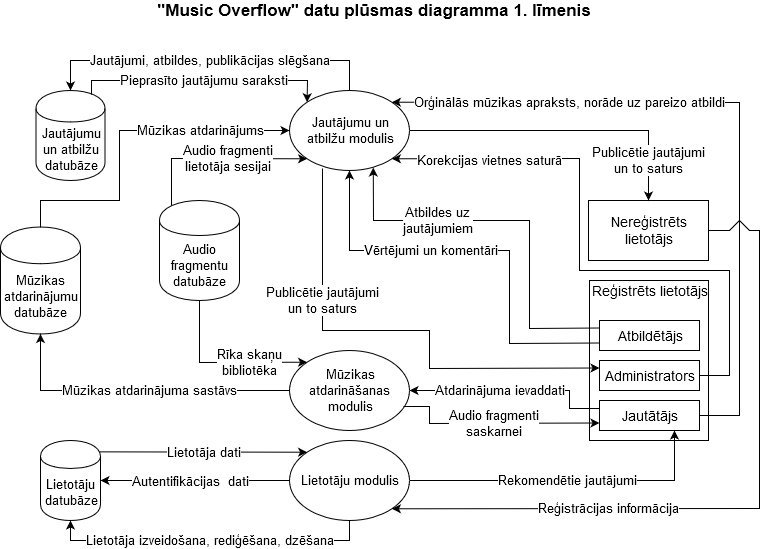
\includegraphics[scale=0.5]{DPD1.png}
	\caption{Datu plūsmas 1. līmeņa diagramma}
	\label{fig:dpd_1}
\end{center}
\end{figure}

\subsubsection{Mūzikas atdarināšanas modulis}

\begin{figure}[H]
\begin{center}
	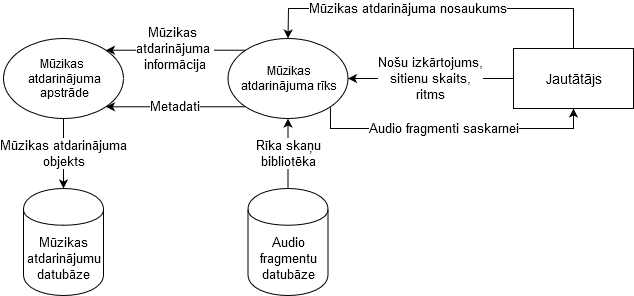
\includegraphics[scale=0.5]{DPD2_1.png}
	\caption{Datu plūsmas 2. līmeņa diagramma mūzikas atdarināšanas modulim}
	\label{fig:dpd_2_1}
\end{center}
\end{figure}

\subsubsection{Jautājumu un atbilžu modulis}

\begin{figure}[H]
\begin{center}
	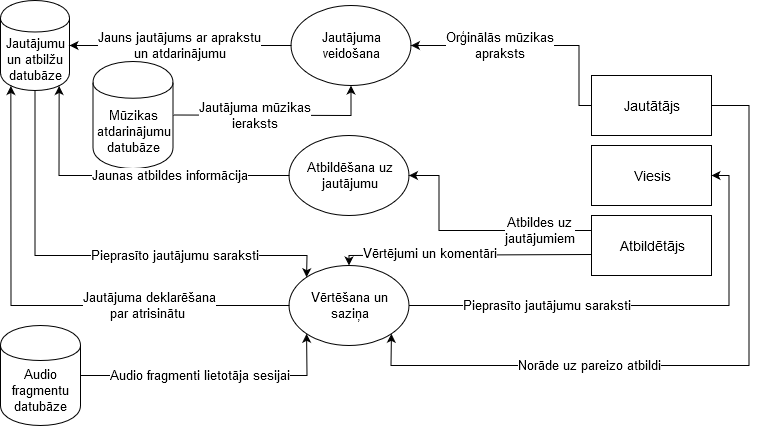
\includegraphics[scale=0.5]{DPD2_2.png}
	\caption{Datu plūsmas 2. līmeņa diagramma jautājumu un atbilžu modulim}
	\label{fig:dpd_2_2}
\end{center}
\end{figure}

\subsubsection{Lietotāju modulis}

\begin{figure}[H]
\begin{center}
	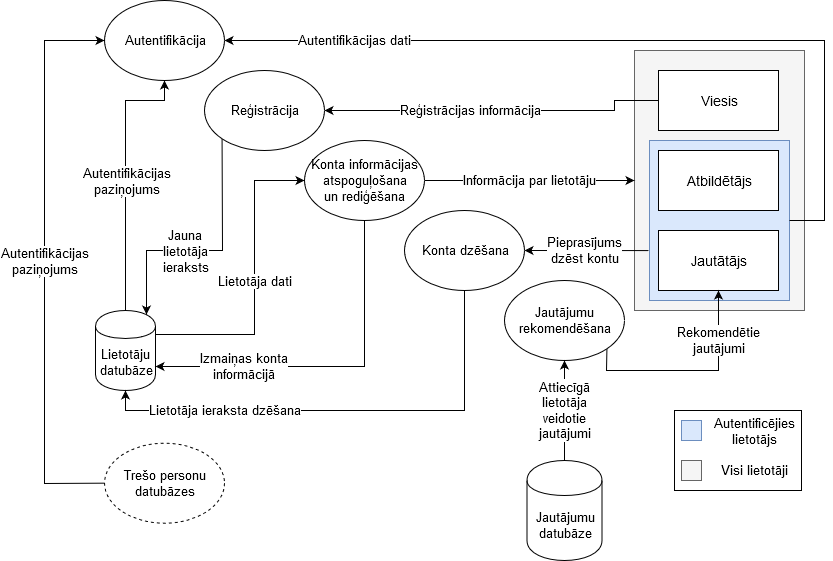
\includegraphics[scale=0.5]{DPD2_3.png}
	\caption{Datu plūsmas 2. līmeņa diagramma lietotāju modulim}
	\label{fig:dpd_2_3}
\end{center}
\end{figure}

\subsection{Nefunkcionālās prasības}

\subsubsection{Veiktspējas prasības}

Sistēmai jāspēj nodrošināt vairāku (vismaz 1000) lietotāju vienlaicīgu sistēmas lietošanu. Apstrādājamo datu apjoms, uz apstrādes ilgumu ierobežojošiem laika limitiem.

\subsubsection{Drošība}

Katram lietotājam būs parole, kura neļaus nepiederošām personām patvaļīgi piekļūt pie sistēmas. Ar autortiesībām aizsargā oriģinālās melodijas autora darbu pret neatļautu lietošanu.

\section{Programmatūras projektējuma apraksts}

\subsection{Datu bāzes projektējums}

Salīdzinot ar konceptuālo datu bāzes modeli (skat. ~\ref{fig:db_konceptualais}), loģiskajā modelī, kas redzams ~\ref{fig:db_logiskais} diagrammā, lai risinātu daudz-pret-daudz relāciju, ir nepieciešamība pēc vēl divām papildus tabulām - ``LietotajsKomentarsVertejums'' un ``LietotajsAtbildeVertejums''.

\begin{figure}[H]
\begin{center}
	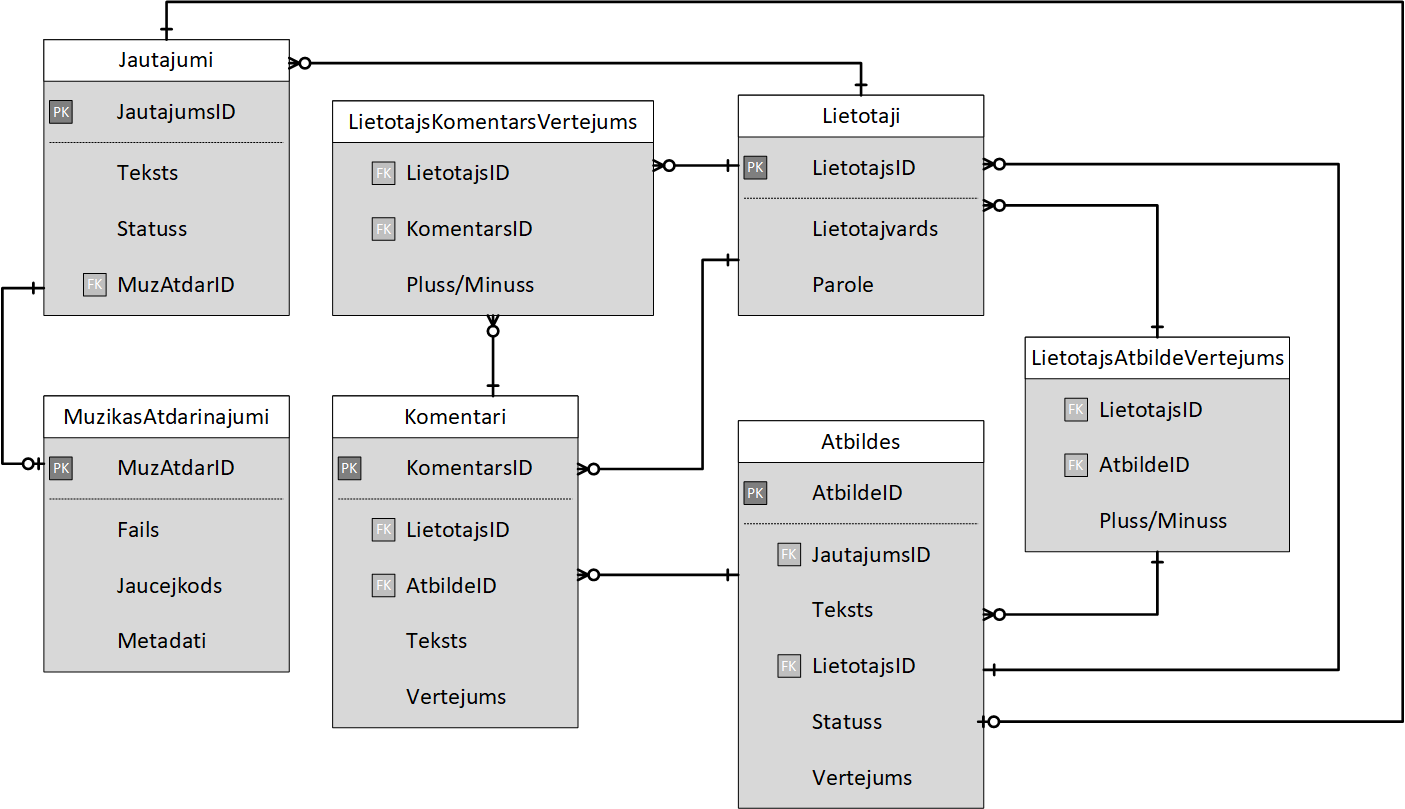
\includegraphics[scale=0.4]{DB_logical.png}
	\caption{Datu bāzes loģiskais modelis}
	\label{fig:db_logiskais}
\end{center}
\end{figure}

\subsection{Daļējs funkciju projektējums}

Programmai tiks izmantota Klienta-Servera tīkla arhitektūra. Uz servera notiks ievadīto datu apstrāde un mūzikas failu ģenerācija, kā arī datu saglabāšana datubāzē, savukārt klienta pusē notiks ģenerējamās melodijas metadatu izveide (skat. ~\ref{fig:deployment_diagram} diagrammu).

\begin{figure}[H]
\begin{center}
	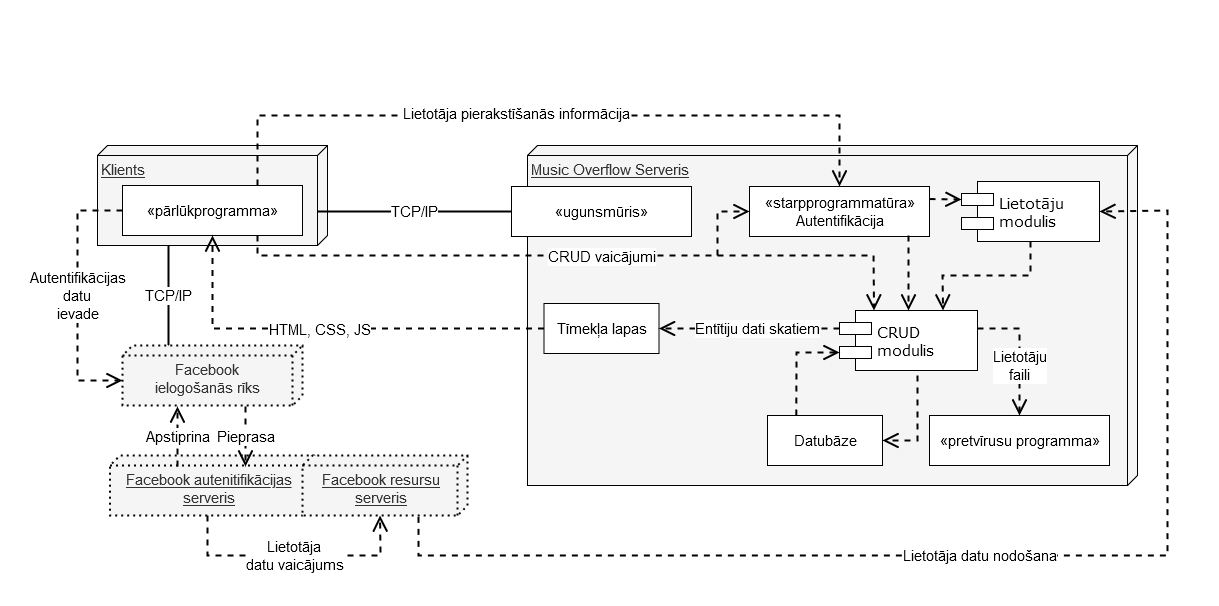
\includegraphics[scale=0.35]{DeploymentDiagram.png}
	\caption{Izvietošanas diagramma}
	\label{fig:deployment_diagram}
\end{center}
\end{figure}

Programmatūra tiks izstrādāta izmantojot ``Modelis-Skats-Kontrolieris'' projektēšanas šablonu. No pārlūkprogrammā ievadītās adreses tiek izsecināts, kurš kontrolieris un kura metode tiek izsaukta. Kontroliera metode apstrādā modeļus, kuri modelē ierakstus datubāzē. Atkarībā no metodes rezultāta, lietotājam tiek parādīta jauna lapa, vai arī tiek izsaukta cita kontroliera metode. Piemērs, kā tas strādā, redzams ~\ref{fig:routing} diagrammā. 

\begin{figure}[H]
\begin{center}
	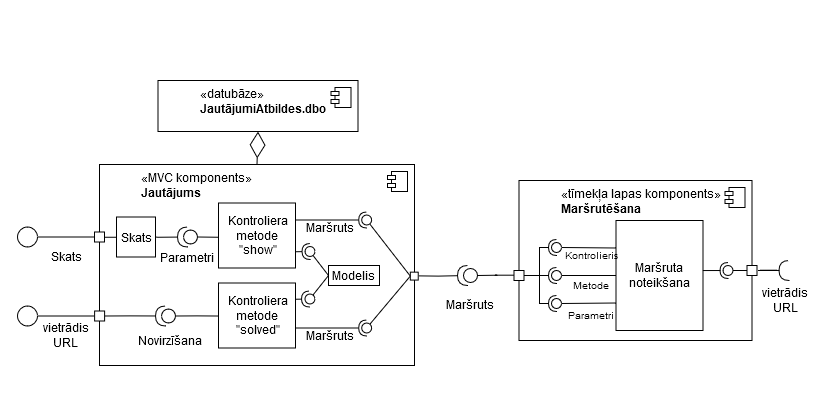
\includegraphics[scale=0.5]{routing.png}
	\caption{Maršrutēšanas diagramma}
	\label{fig:routing}
\end{center}
\end{figure}

Lietotāju autorizācija programmā notiek izmantojot Facebook autorizāciju. Tas ļauj izvairīties no lietotāju paroļu uzglabāšanas, tādējādi uzlabojot programmatūŗas drošību. Tās darbības princips redzams ~\ref{fig:oauth_flow} attēlā.

\begin{figure}[H]
\begin{center}
	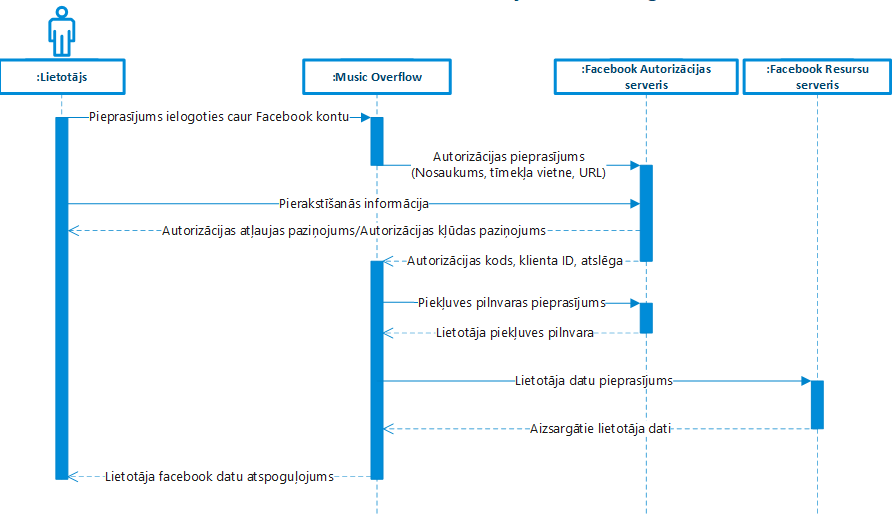
\includegraphics[scale=0.6]{Oauth_flow.png}
	\caption{Autorizācijas diagramma}
	\label{fig:oauth_flow}
\end{center}
\end{figure}

~\ref{fig:activity_diagram} attēlā redzams, kā lietotājs var izveidot melodiju. Pēc melodijas izveides, lietotājam ir iespēja vai nu aplūkot komentārus, vai arī aplūkot informāciju par melodiju.

\begin{figure}[H]
\begin{center}
	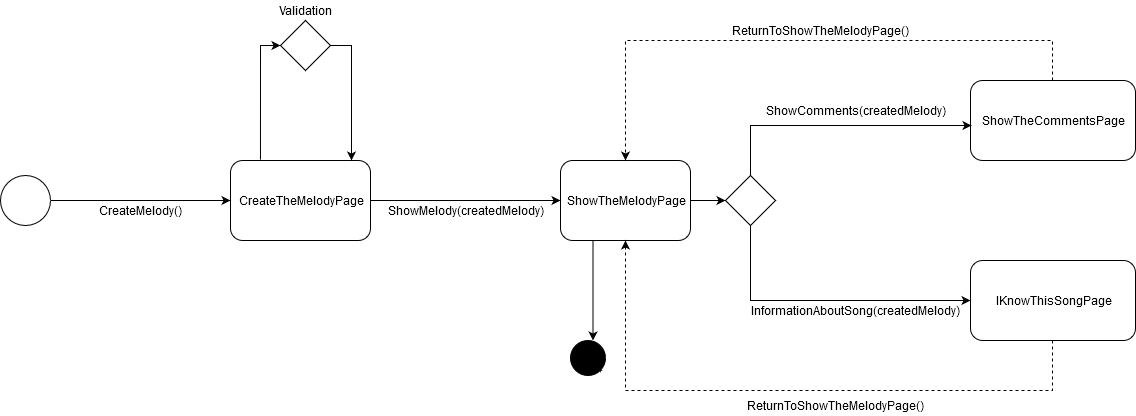
\includegraphics[width=\linewidth,scale=0.5]{ActivityDiagram.png}
	\caption{Aktivitāšu diagramma}
	\label{fig:activity_diagram}
\end{center}
\end{figure}

\subsection{Daļējs lietotāja saskarņu projektējums}

Lietotāja komunikācija ar lietotni notiek, izmantojot pārlūkprogrammu. Ritma ievadei ir nepieciešams tastatūras taustiņš, kur šīs ievades garums ir 30 sekundes.

\pagebreak

\section*{Izmantotā literatūra un avoti}
\addcontentsline{toc}{section}{Izmantotā literatūra un avoti}

\pagebreak

\textbf{\large Dokumentārā lapa}

\end{document}